\section{Backtest}\label{sec:backtest}

If general-election favourites are underpriced, buying them should have paid. This section checks that looking
backwards, on the two general-election nights in the data: 5 November 2024 and the midterms of 3 November 2026. It was
not part of the pre-registration, every rule in it was chosen after seeing the results, and it is included for
discussion rather than as evidence.

\paragraph{What a bet is.} \$100 on the favourite of every US contest with a usable price at the snapshot, held until
the market settled. On Kalshi a bet costs the actual asking price at the snapshot plus the taker fee of 7\% of the price
times one minus the price. On Polymarket only a recorded price is available, so buying is assumed to cost 1 cent more,
plus the taker fee of 4\% of the price times one minus the price from 30 March 2026; there was no fee in 2024. Unlike
Sections~\ref{sec:data} to~\ref{sec:results}, the bets include favourites priced above 95\% and contests in Georgia,
Louisiana and Mississippi, since those bets still settle. That gives 97 bets on Kalshi and 91 on Polymarket in 2024,
and 547 and 419 on the midterms. Intervals resample states, as in Section~\ref{sec:results}.

\subsection{Buying every favourite earns little}

Buying every favourite returned 0.9\% per bet on Kalshi's midterms and 3.0\% on Polymarket's, after costs, and both
intervals include zero (Table~\ref{tab:backtest}). In 2024 the returns were 3.5\% on Kalshi and 7.3\% on Polymarket;
the Polymarket figure benefits from a night on which only 3 of 91 favourites lost, and from the absence of fees.

Two things eat the profit (Figure~\ref{fig:bt_bands}). Close races, with favourites priced between 50\% and 70\%, lost
money on the midterms: 16.5\% on Kalshi's 48 bets and 3.8\% on Polymarket's 34. This matches Section~\ref{sec:results},
where close races were priced about right and the underconfidence sat in clear favourites. Costs are also heaviest
there: Kalshi's fee is about 3\% of the price for a 60\% favourite and under 1\% for a 90\% favourite. At the other end,
favourites priced above 95\% almost always won, but each win paid only 1 to 2 cents on the dollar.

\begin{table}[!htbp]
\centering\small\setlength{\tabcolsep}{4.5pt}
\caption{The backtest: \$100 on every favourite of a group, after costs. Return is profit per \$100 staked, with a 95\%
interval from resampling states. When every bet in a group won, the interval cannot reach below zero, however few the
bets. The last row of each platform takes the best price window of 2024 (Figure~\ref{fig:bt_windows}) and applies it to
the midterms.}\label{tab:backtest}
\begin{tabular}{llL{2.9cm}rrrlr}
\toprule
 & Night & Rule & Bets & Upsets & Return, \% & 95\% interval & Profit \\
\midrule
Kalshi & 2024 & Every favourite & 97 & 12 & $+3.5$ & $-5.9$ to $+12.8$ & \$339 \\
 & & At or above 70\% & 68 & 1 & $+5.9$ & $+1.5$ to $+9.0$ & \$400 \\
 & & 85--90\% & 6 & 0 & $+11.7$ & $+10.6$ to $+12.7$ & \$70 \\
\addlinespace
 & Midterms & Every favourite & 547 & 36 & $+0.9$ & $-3.5$ to $+5.0$ & \$481 \\
 & & At or above 70\% & 499 & 13 & $+2.6$ & $-0.4$ to $+5.0$ & \$1{,}275 \\
 & & 85--90\% & 29 & 1 & $+8.0$ & $-0.1$ to $+12.5$ & \$232 \\
 & & 2024's best window, 75--85\% & 47 & 8 & $+0.5$ & $-27.3$ to $+20.5$ & \$24 \\
\midrule
Polymarket & 2024 & Every favourite & 91 & 3 & $+7.3$ & $+1.5$ to $+12.9$ & \$663 \\
 & & At or above 70\% & 81 & 2 & $+2.9$ & $-3.3$ to $+7.0$ & \$234 \\
 & & 85--90\% & 6 & 0 & $+11.8$ & $+10.5$ to $+12.9$ & \$71 \\
\addlinespace
 & Midterms & Every favourite & 419 & 20 & $+3.0$ & $-0.7$ to $+6.6$ & \$1{,}256 \\
 & & At or above 70\% & 385 & 6 & $+3.6$ & $+1.6$ to $+5.5$ & \$1{,}386 \\
 & & 85--90\% & 26 & 1 & $+8.1$ & $-0.3$ to $+12.9$ & \$211 \\
 & & 2024's best window, 60--70\% & 15 & 6 & $-10.9$ & $-53.8$ to $+36.8$ & $-\$164$ \\
\bottomrule
\end{tabular}
\end{table}

\begin{figure}[!htbp]
\centering
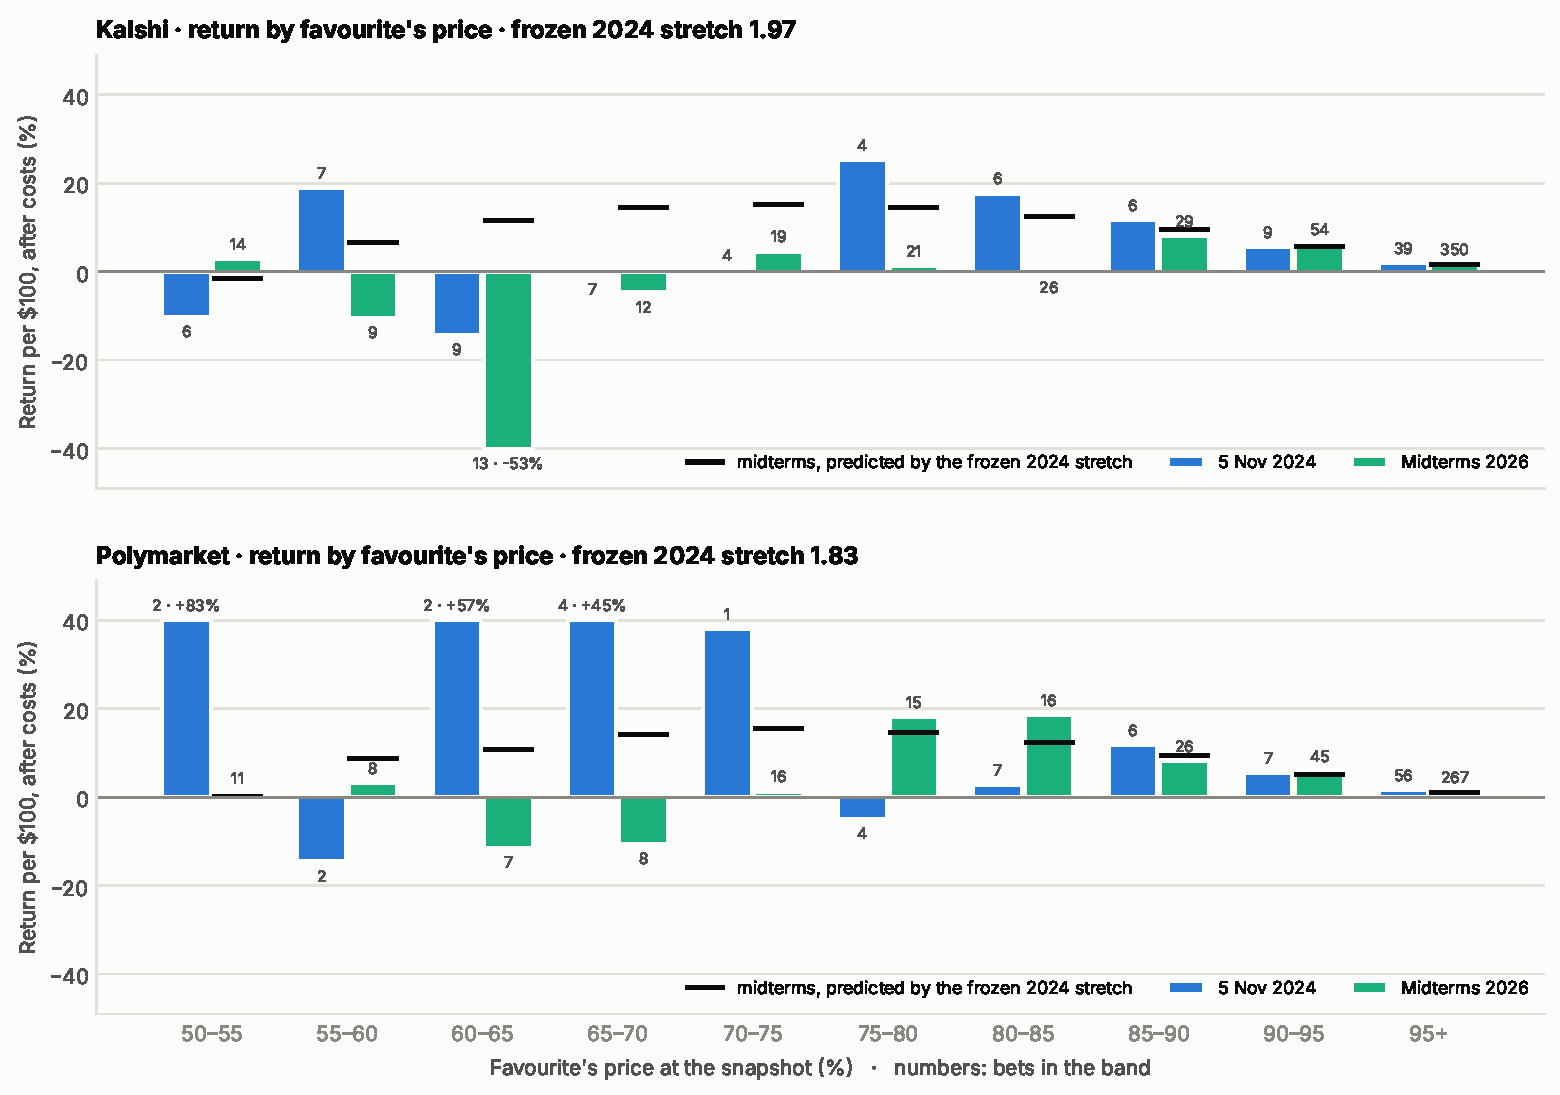
\includegraphics[width=0.9\textwidth]{figures/bt_bands.pdf}
\caption{Return per \$100 after costs, by the favourite's price, on 5 November 2024 (blue) and the midterms (green).
Numbers give the bets in each band; bars beyond $\pm 40\%$ are cut and their value written out. Black marks: the return
the frozen 2024 stretch predicted for the midterm bets in each band, given the prices actually paid. That stretch was
fixed before the vote, so for the midterms the marks are a genuine forecast.}\label{fig:bt_bands}
\end{figure}

\subsection{Favourites above 70\%}

Leaving out the close races fixes most of this. Figure~\ref{fig:bt_thresholds} applies the rule ``buy every favourite
priced at or above a threshold'' for every threshold from 50\% to 95\%. Raising the threshold drops the close races
that lost money, but it also drops bets, and the bets that remain are expensive, with less room to pay. Total profit
therefore peaks in between, and on three of the four platform-nights it peaks close to 70\%: at 71\% on Kalshi's
midterms (\$1{,}401 on 495 bets), at 68\% on Polymarket's midterms (\$1{,}410 on 389) and at 68\% on Kalshi in 2024
(\$596 on 73). At exactly 70\%, the rule returned 2.6\% per bet on Kalshi's midterms and 3.6\% on Polymarket's, the
latter with an interval wholly above zero (1.6\% to 5.5\%). The exception is Polymarket in 2024, where nine of the ten
favourites priced between 50\% and 70\% won, so the most profitable rule was to buy everything.

This is what the bias found in Section~\ref{sec:results} would lead one to expect. A stretch above 1 says favourites
win more often than their prices imply. The gap is zero at 50\%, where the stretch changes nothing, and shrinks again
towards 100\%, where there is no room left. The black marks in Figure~\ref{fig:bt_bands} show the returns the frozen
2024 stretch predicted for the midterm bets. Above 85\%, they are close to what happened: on Kalshi 9.6\% predicted
against 8.0\% earned between 85\% and 90\%, and 5.7\% against 6.3\% between 90\% and 95\%; Polymarket is similar.
Between 60\% and 85\%, the stretch predicted returns of 10\% to 15\%. Kalshi's midterm favourites earned at most
5\% in any of those bands and lost heavily between 60\% and 65\%; Polymarket's fell short of the prediction between
60\% and 75\% and beat it between 75\% and 85\%. A single stretch describes clear favourites well and overstates the
edge in moderately close races.

The margins are thin. Over a whole night, buying every favourite above 70\% returned 2\% to 4\% per bet on the
midterms, and Kalshi's 2024 markets settled only in January 2025, tying the money up for about two months.

\begin{figure}[!htbp]
\centering
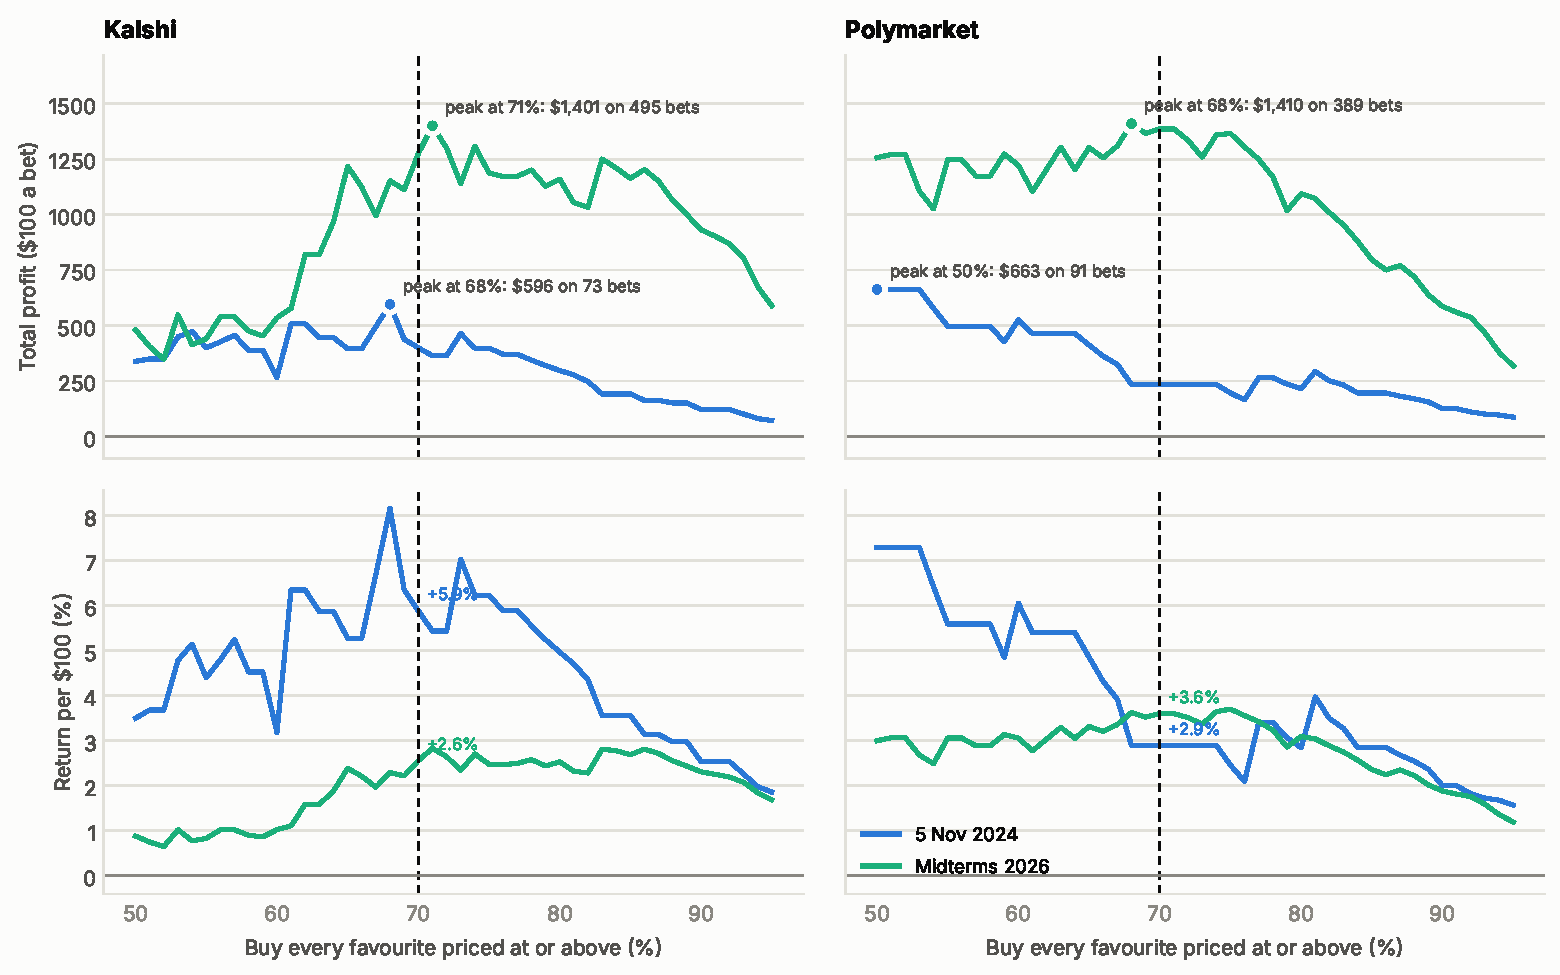
\includegraphics[width=0.86\textwidth]{figures/bt_thresholds.pdf}
\caption{Buying every favourite priced at or above a threshold, for thresholds from 50\% to 95\% in steps of one point.
Top: total profit at \$100 a bet, with each night's peak marked. Bottom: return per \$100. Dashed line: 70\%. The
jagged lines show how much a single upset moves the result.}\label{fig:bt_thresholds}
\end{figure}

\subsection{The 85--90\% band, and why it is probably overfitted}

The best-paying band that made money on both nights and on both platforms is 85\% to 90\%. Favourites priced there
returned 11.7\% on Kalshi and 11.8\% on Polymarket in 2024, and 8.0\% and 8.1\% on the midterms. Only 2 of their 67
bets lost.

It would be a mistake to read this as a strategy. There are few bets: six on each platform in 2024, where one more
upset would have turned the profit into a loss, and 29 and 26 on the midterms, where the intervals reach below zero.
The 2024 intervals look narrow only because every bet won, and resampling bets that all won can never produce a loss.
Nothing in the bias singles out this band either: the frozen stretch predicted larger returns between 65\% and 85\%
than between 85\% and 90\% (Figure~\ref{fig:bt_bands}).

More importantly, the band was found by searching. Figure~\ref{fig:bt_windows} shows every price window with edges at
5-point steps, 55 of them per platform and night. With that many to choose from, some window will look excellent on any
night, and which one it is changes from night to night: 75--85\% for Kalshi in 2024 (21\% on 10 bets), 85--90\% for
Kalshi's midterms, 60--70\% for Polymarket in 2024 (49\% on 6 bets) and 80--85\% for Polymarket's midterms (19\% on 16
bets). A trader who had picked the best window of 2024 and bought it on the midterms would have made 0.5\% on Kalshi and
lost 10.9\% on Polymarket (Table~\ref{tab:backtest}). Every strategy looks good in a backtest once it has been adjusted
enough, and the 85--90\% band was chosen by looking at the same two nights on which it is evaluated.

\begin{figure}[!htbp]
\centering
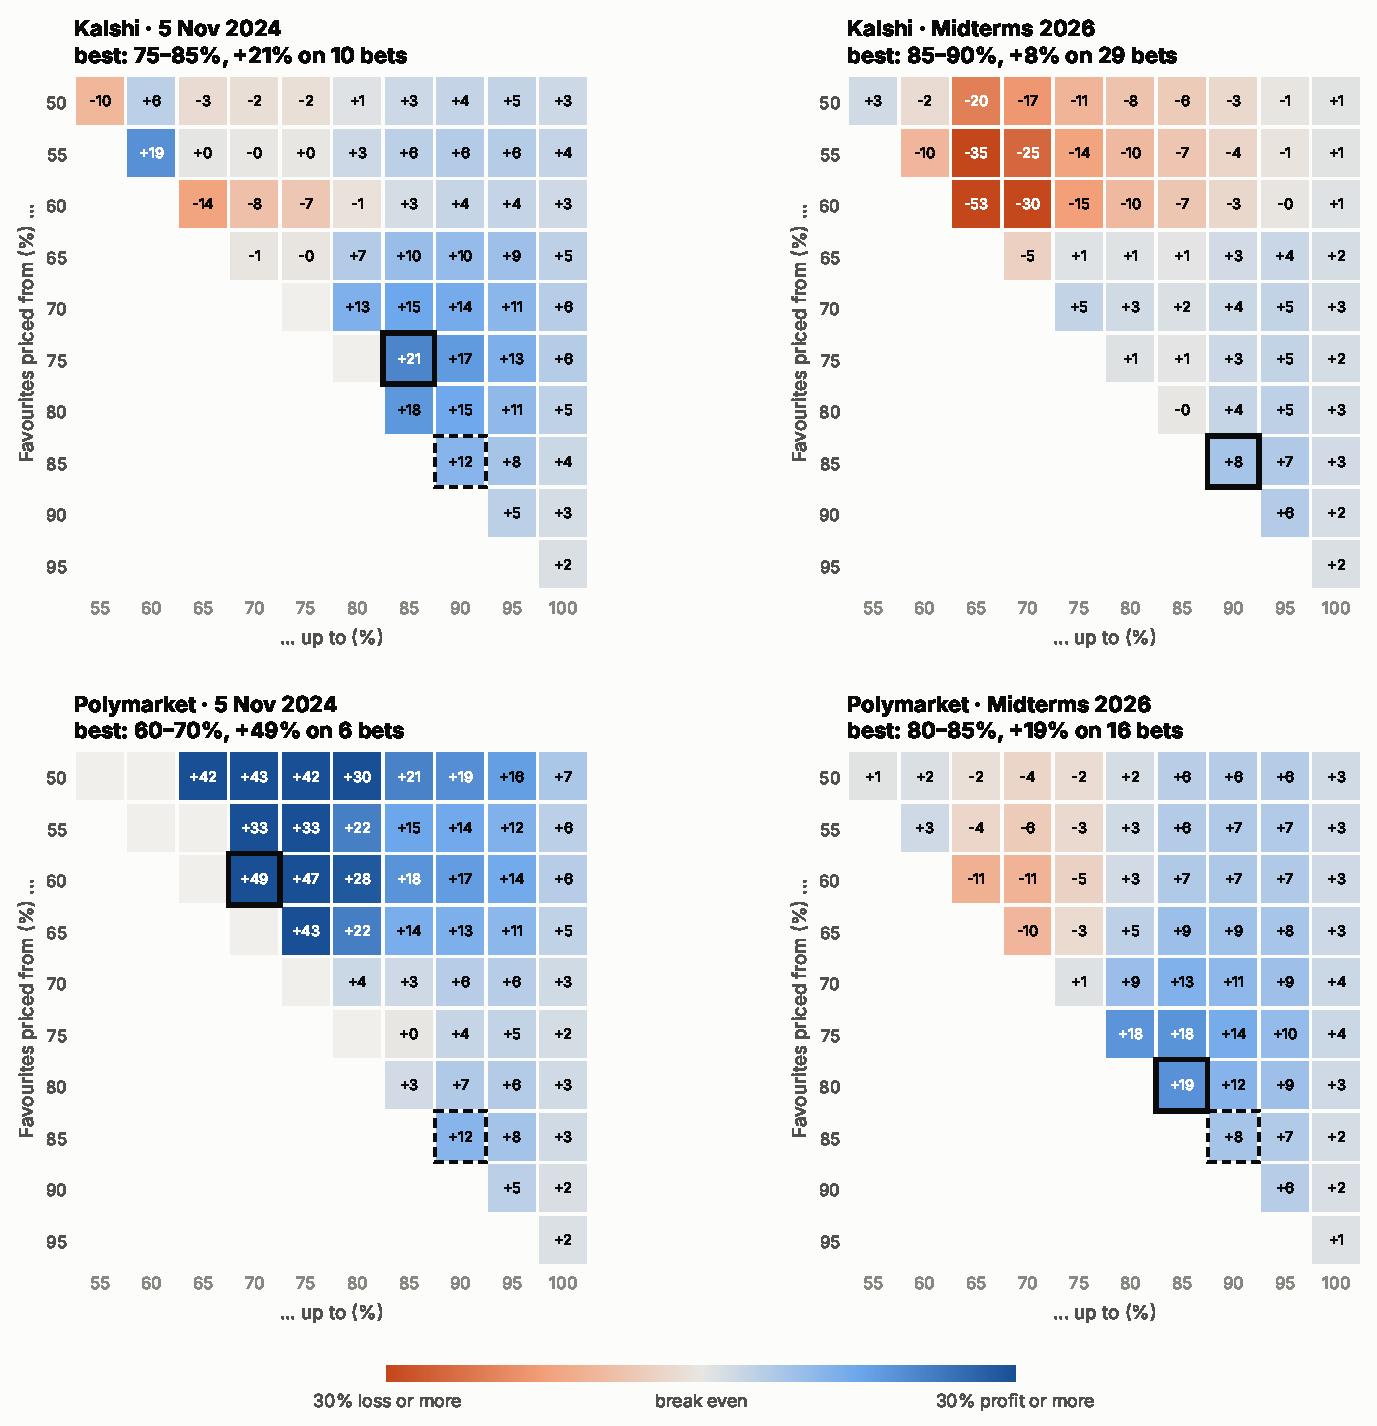
\includegraphics[width=0.8\textwidth]{figures/bt_windows.pdf}
\caption{Every price window: buy every favourite priced from the row's value up to the column's value (the last column
includes everything up to 100\%). Colour and number: return per \$100 after costs. Blank: fewer than five bets. Solid
outline: the best window on that night. Dashed outline: 85--90\% (on Kalshi's midterms the two coincide).}
\label{fig:bt_windows}
\end{figure}

\subsection{What the backtest can and cannot say}

Beyond the search problem, the results flatter the strategy in several ways. Contests enter only if they settled with
one of the two listed candidates winning, and the 40 midterm races still unsettled lean towards those in which the
favourite struggled. Bets on one night are not independent: a national swing moves every race at once, and resampling
states does not capture that, so the two nights are in effect two observations. The Kalshi asking price is good only
for the first few contracts, and the depth of the order book behind it was not recorded. No interest is counted on the
money tied up until settlement.

What the backtest does support is the shape of the opportunity, if the underconfidence persists: the money is in clear
favourites rather than in close races, it fades above 95\%, and after costs it is a few percent per bet. Whether a rule
such as ``buy every favourite above 70\%'' works can only be settled the way the main hypothesis was: by fixing it
before the next general election and checking it afterwards.
